\section{4. Cài đặt và giao diện}

\subsection{4.1. Công nghệ}

Toàn bộ chương trình viết bằng \textbf{Python 3.11} {[}9{]}. Giao diện 3D dùng \textbf{Ursina 7.0.0} {[}10{]}, một engine game chạy trên \textbf{Panda3D 1.10.16} {[}11{]}. Nhóm chọn Ursina vì ba lý do:

\begin{enumerate}
\def\labelenumi{\arabic{enumi}.}
\tightlist
\item
  Cùng ngôn ngữ với engine và thuật toán, nên giao diện gọi thẳng hàm luật chơi của nhóm, không phải viết lại luật hay dựng thêm một lớp giao tiếp.
\item
  Bản demo đầu tiên dùng giao diện web (Three.js {[}14{]}, phông chữ Baloo 2 và Nunito {[}15{]}) gọi engine qua server HTTP. Cách đó đẹp hơn nhưng phải giữ thêm server, API và mã JavaScript; khi chuyển sang Ursina, nhóm không dùng phần này nữa.
\item
  Ursina đủ để dựng bàn 3D có hoạt ảnh lăn, tách, ghép và rơi. Một nhóm khóa trước cùng môn đã dùng Ursina cho đề tài này; nhóm tham khảo danh sách lỗi hay gặp của họ, không dùng lại code {[}8{]}.
\end{enumerate}

Ursina chạy trên Panda3D, mà Panda3D thường ra bản cho phiên bản Python mới chậm hơn. Vì vậy cả nhóm dùng chung Python 3.11, và \texttt{requirements.\allowbreak{}txt} ghim đúng phiên bản \texttt{ursina==7.\allowbreak{}0.\allowbreak{}0}, \texttt{panda3d==1.\allowbreak{}10.\allowbreak{}16} để máy chấm không cài nhầm bản mới hơn.

\subsection{4.2. Cấu trúc thư mục và kiến trúc}

\begin{verbatim}
Source/
  main.py            điểm vào: mở giao diện
  bloxorz/           engine luật chơi (state.py, level.py, rules.py, problem.py, costs.py, maze.py)
  solvers/           BFS, DFS, UCS, A*, heuristic; runner.py chạy solver ở tiến trình riêng
  gui/               giao diện Ursina (app.py, board_view.py, block_view.py, hud.py, camera_controller.py,
                     popup.py, theme.py, meshes.py, anim.py; fonts/)
  levels/original/   33 màn gốc (JSON)
  tests/             unit test
\end{verbatim}

Chương trình chia thành ba lớp, phụ thuộc theo một chiều:

{\def\LTcaptype{none} % do not increment counter
\begin{longtable}[]{@{}
  >{\raggedright\arraybackslash}p{(\linewidth - 4\tabcolsep) * \real{0.2639}}
  >{\raggedright\arraybackslash}p{(\linewidth - 4\tabcolsep) * \real{0.4306}}
  >{\raggedright\arraybackslash}p{(\linewidth - 4\tabcolsep) * \real{0.3056}}@{}}
\toprule\noalign{}
\begin{minipage}[b]{\linewidth}\raggedright
\textbf{Package}
\end{minipage} & \begin{minipage}[b]{\linewidth}\raggedright
\textbf{Được dùng}
\end{minipage} & \begin{minipage}[b]{\linewidth}\raggedright
\textbf{Không được dùng}
\end{minipage} \\
\midrule\noalign{}
\endhead
\bottomrule\noalign{}
\endlastfoot
\texttt{bloxorz/\allowbreak{}} (engine) & thư viện chuẩn & \texttt{solvers}, \texttt{gui}, \texttt{ursina} \\
\texttt{solvers/\allowbreak{}} & \texttt{bloxorz} & \texttt{gui}, \texttt{ursina} \\
\texttt{gui/\allowbreak{}} & \texttt{bloxorz}, và từ \texttt{solvers} chỉ \texttt{ALGORITHMS} cùng module \texttt{runner} & gọi thẳng thuật toán \\
\end{longtable}
}

Quy tắc này có hai hệ quả. Thứ nhất, \textbf{chơi tay và thuật toán dùng chung một hàm luật}: mỗi nước đi, dù do người bấm phím hay do khối tự lăn theo lời giải, đều qua \texttt{rules.\allowbreak{}step(level, state, action)}; giao diện không tự tính luật. Thứ hai, engine, thuật toán và test chạy được trên máy chưa cài Ursina, nên thực nghiệm và kiểm thử không phụ thuộc giao diện.

\texttt{step()} trả về \texttt{StepResult} gồm trạng thái mới, kết quả (\texttt{ok}, \texttt{fell}, \texttt{won}), vị trí ngay sau khi lăn (dùng cho hoạt ảnh) và danh sách sự kiện theo thứ tự xảy ra: công tắc tác động, ô dễ vỡ vỡ, tách, ghép, rơi, thắng. Giao diện chỉ đọc các trường này để vẽ.

Các file của \texttt{gui/\allowbreak{}} chia việc như sau:

{\def\LTcaptype{none} % do not increment counter
\begin{longtable}[]{@{}
  >{\raggedright\arraybackslash}p{(\linewidth - 2\tabcolsep) * \real{0.3056}}
  >{\raggedright\arraybackslash}p{(\linewidth - 2\tabcolsep) * \real{0.6944}}@{}}
\toprule\noalign{}
\begin{minipage}[b]{\linewidth}\raggedright
\textbf{File}
\end{minipage} & \begin{minipage}[b]{\linewidth}\raggedright
\textbf{Việc}
\end{minipage} \\
\midrule\noalign{}
\endhead
\bottomrule\noalign{}
\endlastfoot
\texttt{board\_\allowbreak{}view.\allowbreak{}py} & Dựng bàn từ \texttt{Level}: mỗi ô một khối hộp; cầu đổi màu khi mở hoặc đóng; ô dễ vỡ rơi khi vỡ; viền ô đích nhấp nháy \\
\texttt{block\_\allowbreak{}view.\allowbreak{}py} & Vẽ khối hoặc hai khối con theo \texttt{State}; hoạt ảnh lăn, tách, ghép, rơi \\
\texttt{hud.\allowbreak{}py} & Các nút, lưới chọn màn, khung kết quả và bảng So sánh \\
\texttt{camera\_\allowbreak{}controller.\allowbreak{}py} & Góc nhìn: các nấc nghiêng, góc nhìn đỉnh, thu phóng, căn bàn khi khung kết quả hiện (mục 4.7) \\
\texttt{app.\allowbreak{}py} & Cửa sổ, phím, vòng \texttt{update()}; nối phím với \texttt{rules.\allowbreak{}step()} và nút với \texttt{runner} \\
\texttt{popup.\allowbreak{}py} & Hộp kết thúc màn (thắng, rơi) với các nút hành động tiếp theo; kéo thả được \\
\texttt{theme.\allowbreak{}py} & Font Be Vietnam Pro (thư mục \texttt{fonts/\allowbreak{}}) và thẻ kiểu kính mờ dùng chung \\
\texttt{meshes.\allowbreak{}py} & Mesh hộp vát cạnh cho ô và khối, tạo một lần rồi dùng lại \\
\texttt{anim.\allowbreak{}py} & Hoạt ảnh hẹn giờ dừng được, an toàn khi đổi màn (lỗi của Ursina 7, mục 4.5) \\
\end{longtable}
}

Tọa độ: ô ở hàng r, cột c có tâm tại x = c, z = −r trong không gian 3D, trục y hướng lên. Camera luôn đặt phía z âm, nhìn xuống bàn, nên phím ↑ (hàng giảm) luôn đẩy khối ra xa người xem.

\subsection{4.3. Cài đặt và chạy}

\begin{verbatim}
cd Source
python -m venv .venv
.venv\Scripts\activate
python -m pip install -r requirements.txt
python main.py          # mở trang chủ; python main.py 17 mở thẳng màn 17
python -m unittest discover -v
\end{verbatim}

Thuật toán chạy ở tiến trình riêng bằng \texttt{multiprocessing} kiểu \texttt{spawn}, nên \texttt{main.\allowbreak{}py} có \texttt{if \_\allowbreak{}\_\allowbreak{}name\_\allowbreak{}\_\allowbreak{} == "\_\allowbreak{}\_\allowbreak{}main\_\allowbreak{}\_\allowbreak{}":} (bắt buộc trên Windows). \texttt{main.\allowbreak{}py} chỉ import giao diện bên trong hàm \texttt{main()}: tiến trình con nạp lại file này khi khởi động, và nếu Ursina được import ở đầu file thì mỗi lần bấm Giải sẽ chậm thêm khoảng một giây.

Đã thử cài theo các lệnh trên trong một môi trường ảo mới trên Windows 11: \texttt{pip} cài đúng hai phiên bản đã ghim, toàn bộ test qua và cửa sổ mở được.

\subsection{4.4. Bàn chơi và các loại ô}

Các ảnh trong chương được chụp ngày 31/10, trước khi thêm trang chủ, nên thanh điều hướng trong ảnh chưa có nút Trang chủ; các phần còn lại giống giao diện hiện tại. Hình 4.1 là màn 23, màn duy nhất trong 33 màn gốc có đủ 9 loại ô. Mỗi loại ô có màu hoặc hình riêng (Bảng 4.1). Góc trên bên trái ghi tên màn, nhóm độ khó, số bước tối ưu tham khảo và số bước đã đi; các nút ở bên phải; dòng dưới cùng tóm tắt các phím hay dùng (F1 mở bảng đầy đủ). Phím G hoặc nút ``Chú giải'' mở bảng chú giải các loại ô (Hình 4.11). Chữ dùng font Be Vietnam Pro {[}13{]}, thiết kế cho tiếng Việt nên dấu rõ ở cỡ nhỏ.

\begin{figure}
\centering
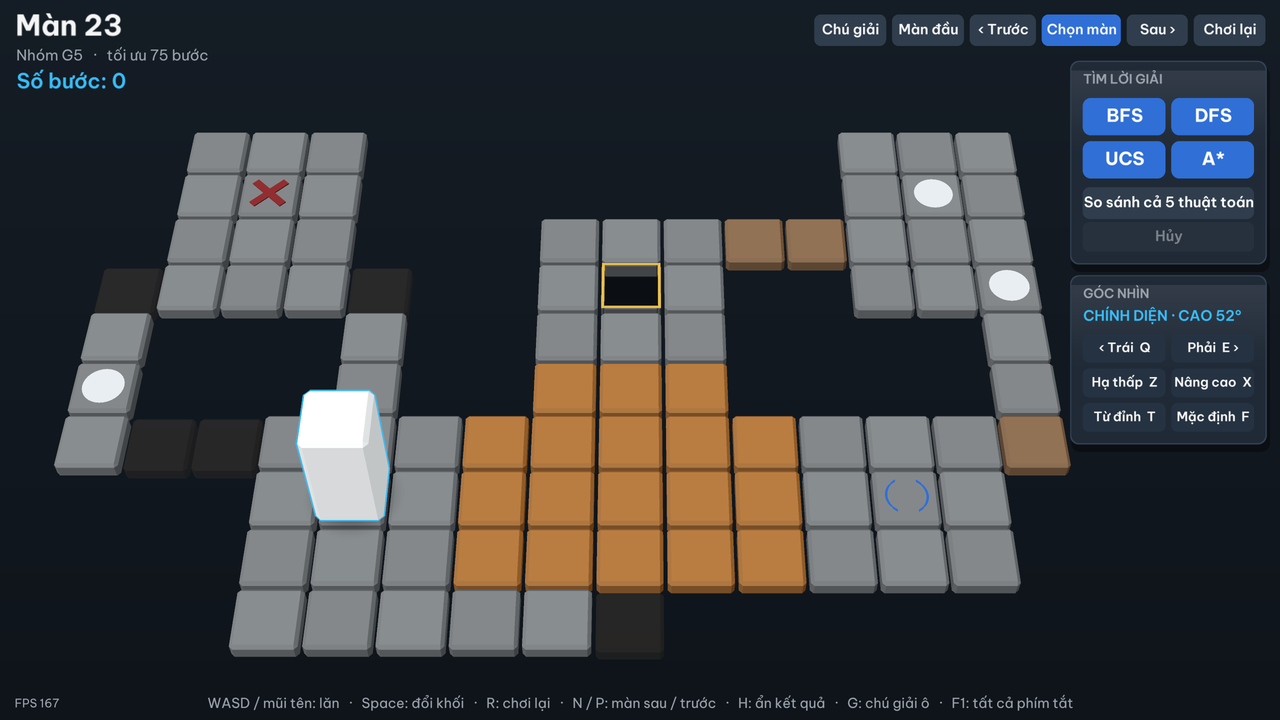
\includegraphics[width=0.86\linewidth,height=\textheight,keepaspectratio,alt={Hình 4.1}]{hinh/h4-1-man23-du-loai-o.png}
\caption{Hình 4.1. Màn 23 lúc bắt đầu: đủ 9 loại ô trên cùng một bàn, phân biệt được bằng màu và hình.}
\end{figure}

Bảng chú giải (Hình 4.11) là một lớp phủ giữa màn hình như bảng phím tắt: mỗi mục có một ô mẫu, tên và cách ô hoạt động theo luật. Ô mẫu vẽ bằng đúng màu và ký hiệu của bàn (lấy từ \texttt{board\_\allowbreak{}view.\allowbreak{}COLORS}), nên đổi màu ô trên bàn thì chú giải đổi theo. Khi bảng đang mở, phím lăn và Enter bị bỏ qua; G hoặc Esc đóng bảng.

\begin{figure}
\centering
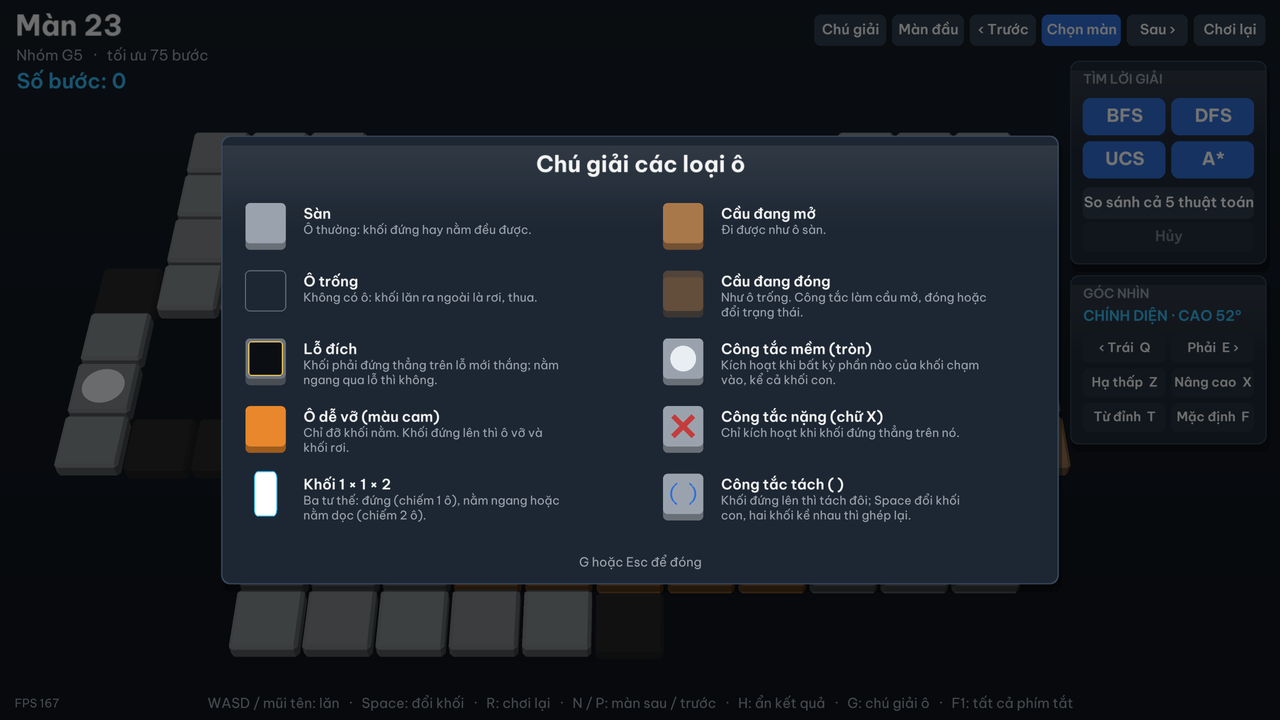
\includegraphics[width=0.86\linewidth,height=\textheight,keepaspectratio,alt={Hình 4.11}]{hinh/h4-11-chu-giai.png}
\caption{Hình 4.11. Bảng chú giải các loại ô (phím G) trên màn 23: cột trái là ô và khối, cột phải là cầu và ba loại công tắc.}
\end{figure}

\begin{longtable}[]{@{}
  >{\raggedright\arraybackslash}p{(\linewidth - 4\tabcolsep) * \real{0.2500}}
  >{\raggedright\arraybackslash}p{(\linewidth - 4\tabcolsep) * \real{0.2612}}
  >{\raggedright\arraybackslash}p{(\linewidth - 4\tabcolsep) * \real{0.4888}}@{}}
\caption{\textbf{Bảng 4.1.} Cách vẽ từng loại ô.}\tabularnewline
\toprule\noalign{}
\begin{minipage}[b]{\linewidth}\raggedright
\textbf{Ô}
\end{minipage} & \begin{minipage}[b]{\linewidth}\raggedright
\textbf{Ký hiệu trong file màn}
\end{minipage} & \begin{minipage}[b]{\linewidth}\raggedright
\textbf{Cách vẽ}
\end{minipage} \\
\midrule\noalign{}
\endfirsthead
\toprule\noalign{}
\begin{minipage}[b]{\linewidth}\raggedright
\textbf{Ô}
\end{minipage} & \begin{minipage}[b]{\linewidth}\raggedright
\textbf{Ký hiệu trong file màn}
\end{minipage} & \begin{minipage}[b]{\linewidth}\raggedright
\textbf{Cách vẽ}
\end{minipage} \\
\midrule\noalign{}
\endhead
\bottomrule\noalign{}
\endlastfoot
Sàn, ô xuất phát & \texttt{\#}, \texttt{S} & Khối hộp xám \\
Ô trống & \texttt{.\allowbreak{}} & Không vẽ gì \\
Đích & \texttt{G} & Lỗ vuông tối, viền vàng nhấp nháy nhẹ để dễ tìm \\
Ô dễ vỡ & \texttt{F} & Khối hộp cam \\
Công tắc mềm & \texttt{o} & Sàn có đĩa tròn trắng \\
Công tắc nặng & \texttt{x} & Sàn có hình X đỏ \\
Công tắc tách & \texttt{@} & Sàn có hình ``( )'' xanh \\
Cầu mở & \texttt{B} (hoặc \texttt{b} sau khi mở) & Khối hộp màu gỗ \\
Cầu đóng & \texttt{b} (hoặc \texttt{B} sau khi đóng) & Khối hộp sẫm, gần trong suốt, nhìn rõ chỗ có cầu \\
\end{longtable}

Khối 1×1×2 màu trắng có viền xanh sáng để nổi trên sàn xám, và có ba tư thế (Hình 4.2). Kích thước khối nhỏ hơn ô một chút để luôn thấy viền giữa khối và sàn. Ô và khối là hộp vát cạnh, mặt bên tối hơn mặt trên, nên bàn có độ dày mà không cần đèn mạnh. Cảnh không dùng bóng đổ thật: bóng của khối phủ lên ô làm màu ô khó phân biệt, nhất là ô dễ vỡ và cầu đóng. Thay vào đó, dưới mỗi khối có một vệt bóng mềm, nhạt dần khi khối nhấc lên, đủ để thấy khối đang chạm sàn. Cạnh ô và khối được khử răng cưa (multisample 4×).

\begin{figure}
\centering
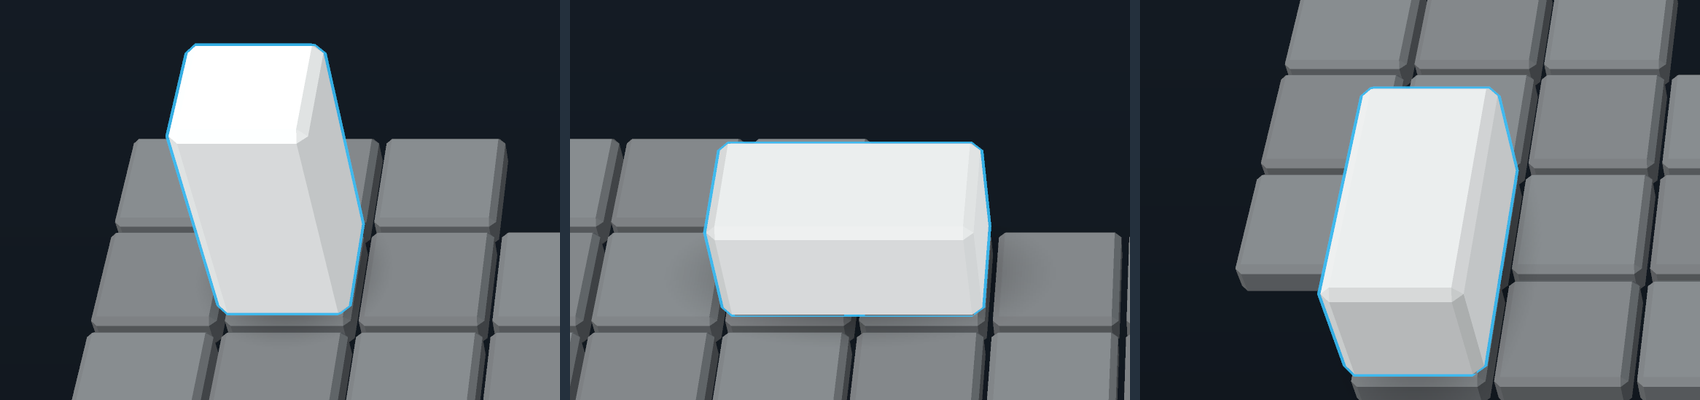
\includegraphics[width=0.86\linewidth,height=\textheight,keepaspectratio,alt={Hình 4.2}]{hinh/h4-2-ba-tu-the.png}
\caption{Hình 4.2. Ba tư thế của khối ở màn 1: đứng chiếm một ô, nằm ngang (sau phím →) và nằm dọc (sau phím ↓) chiếm hai ô.}
\end{figure}

Khi công tắc tác động, cầu bị điều khiển đổi màu dần giữa màu gỗ và màu sẫm, kèm một dòng thông báo cho biết loại công tắc và hiệu ứng (Hình 4.3). Thông báo lấy từ sự kiện \texttt{switch} của engine, không do giao diện tự suy ra.

\begin{figure}
\centering
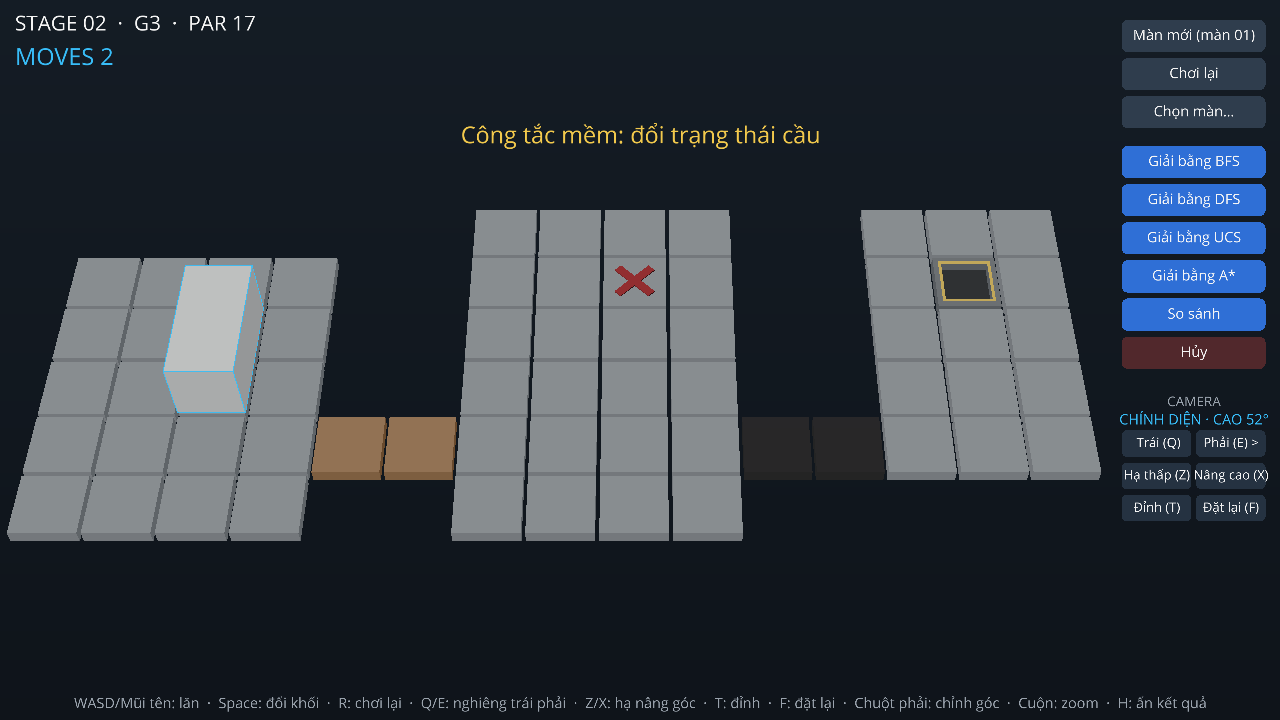
\includegraphics[width=0.86\linewidth,height=\textheight,keepaspectratio,alt={Hình 4.3}]{hinh/h4-3-cong-tac-va-cau.png}
\caption{Hình 4.3. Màn 2, bước 2: khối nằm vừa chạm công tắc mềm nên cặp cầu bên trái mở; cặp cầu bên phải vẫn đóng cho tới khi khối đứng lên công tắc nặng (dấu X đỏ).}
\end{figure}

Khi khối đứng lên công tắc tách, hai khối con bay theo đường vòng cung từ chỗ khối cũ tới hai ô định sẵn (Hình 4.4). Khối con đang điều khiển màu trắng, viền xanh rõ; khối còn lại màu xám, viền mờ; phím Space đổi khối. Engine luôn sắp hai khối con theo thứ tự ô, nên sau mỗi bước, giao diện tìm lại khối vừa đi theo ô mới của nó để giữ đúng khối người chơi đang điều khiển. Hai khối con kề nhau thì tự ghép lại, có thông báo.

\begin{figure}
\centering
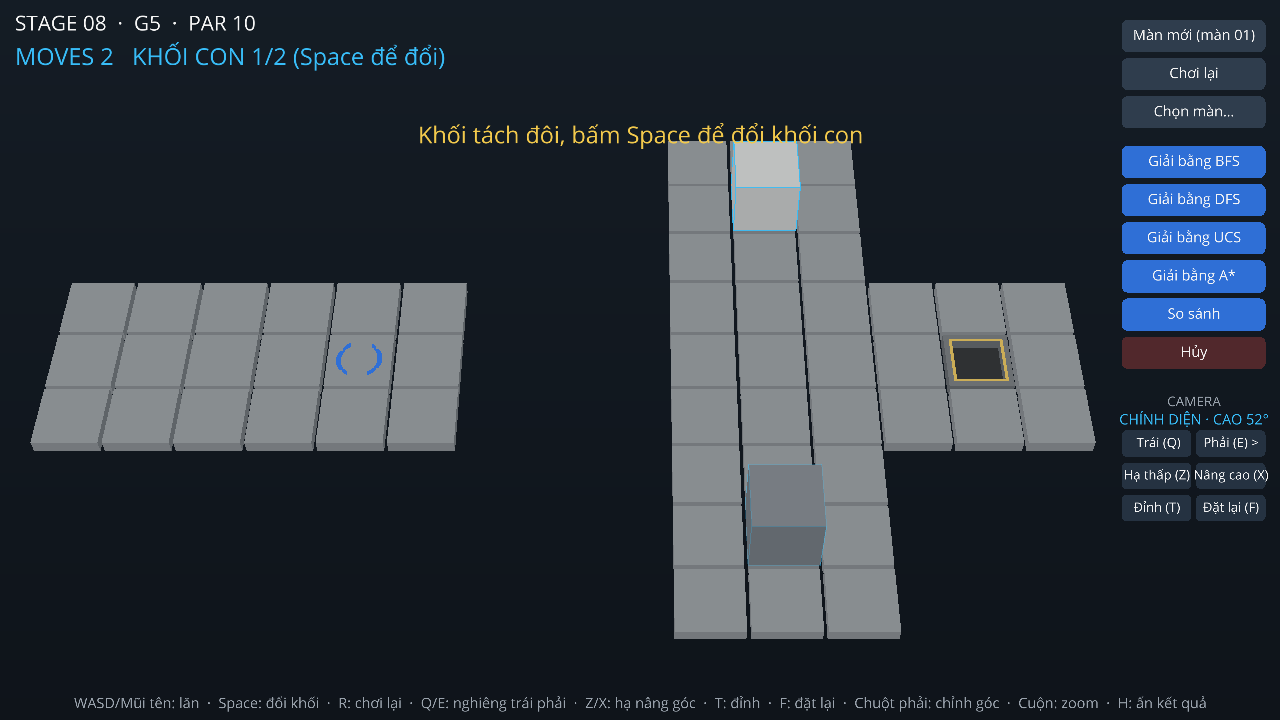
\includegraphics[width=0.86\linewidth,height=\textheight,keepaspectratio,alt={Hình 4.4}]{hinh/h4-4-tach-khoi.png}
\caption{Hình 4.4. Màn 8 sau khi tách: khối con sáng màu là khối đang điều khiển (ghi ``KHỐI CON 1/2'' cạnh số bước).}
\end{figure}

Khối rơi khi chạm ô trống, ra ngoài bàn, vào cầu đóng, hoặc đứng thẳng trên ô dễ vỡ. Giao diện hiện lý do rơi; với ô dễ vỡ, ô cam rơi cùng khối (Hình 4.5) và được dựng lại khi bấm R. Khối nằm mà chỉ một đầu hụt thì đổ nghiêng qua mép ô còn đỡ rồi mới rơi, không xuyên qua sàn; khi đã tách, chỉ khối con bị hụt rơi. Khối mờ dần khi rơi xuống dưới bàn. Việc chọn kiểu đổ chỉ dựa vào hình (ô nào còn tấm đỡ); quyết định có rơi hay không vẫn do \texttt{rules.\allowbreak{}step()}.

\begin{figure}
\centering
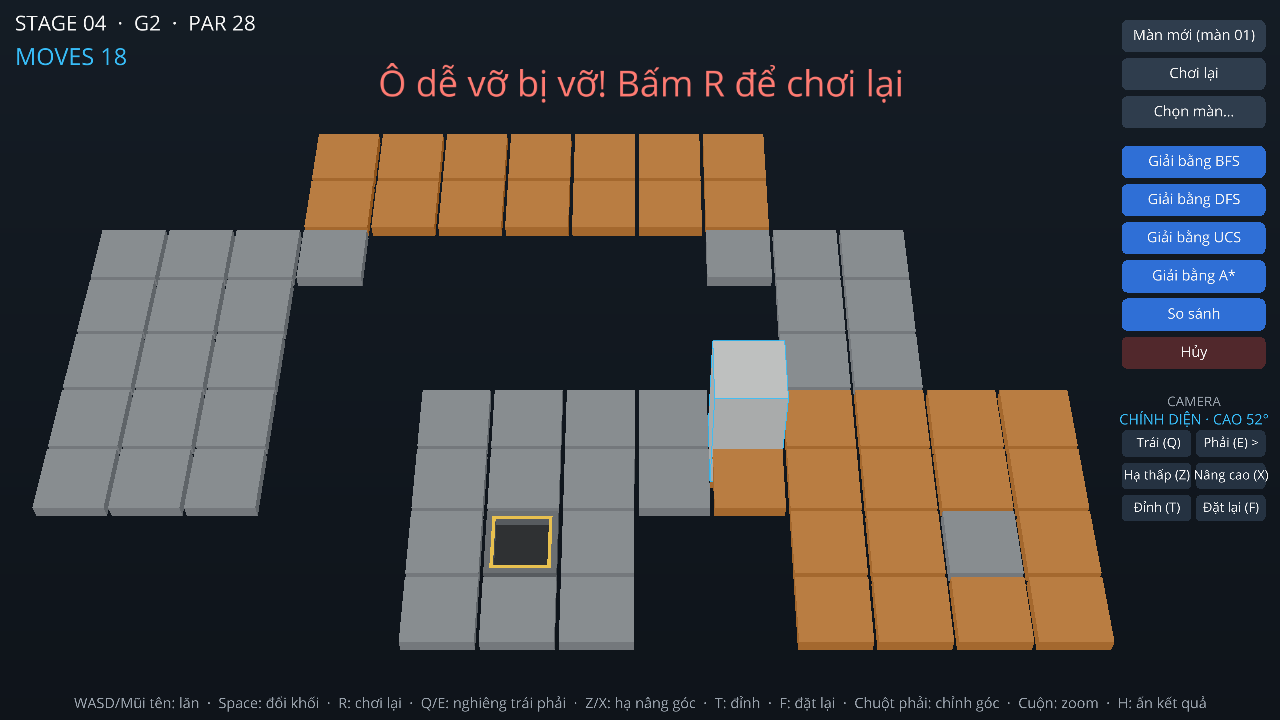
\includegraphics[width=0.86\linewidth,height=\textheight,keepaspectratio,alt={Hình 4.5}]{hinh/h4-5-o-de-vo.png}
\caption{Hình 4.5. Màn 4, bước 18: khối đứng thẳng lên ô dễ vỡ, ô cam vỡ và đang rơi cùng khối (giữa phía dưới); hộp kết thúc (được kéo lên mép trên) nêu đúng lý do thua.}
\end{figure}

\subsection{4.5. Chơi tay}

\textbf{Trang chủ.} Chạy \texttt{python main.\allowbreak{}py} không kèm số màn thì trang chủ hiện ra: bàn 3D của màn 1 xoay chậm phía sau, bên trái là tên game và bốn nút Chơi ngay, Chọn màn, Cách chơi, Thoát (chọn bằng chuột, hoặc bằng phím mũi tên rồi Enter). Nút Cách chơi mở bảng hướng dẫn bốn trang, mỗi trang có một bàn mô phỏng tự chạy: mục tiêu của màn, cách lăn khối, khi nào thì thua, các ô đặc biệt và cách nhờ thuật toán giải. Trong lúc chơi, nút Trang chủ hoặc phím M đưa về trang chủ. Các phím khi chơi:

{\def\LTcaptype{none} % do not increment counter
\begin{longtable}[]{@{}
  >{\raggedright\arraybackslash}p{(\linewidth - 2\tabcolsep) * \real{0.3777}}
  >{\raggedright\arraybackslash}p{(\linewidth - 2\tabcolsep) * \real{0.6223}}@{}}
\toprule\noalign{}
\begin{minipage}[b]{\linewidth}\raggedright
\textbf{Phím}
\end{minipage} & \begin{minipage}[b]{\linewidth}\raggedright
\textbf{Tác dụng}
\end{minipage} \\
\midrule\noalign{}
\endhead
\bottomrule\noalign{}
\endlastfoot
← ↑ → ↓ hoặc W A S D & Lăn khối \\
Space & Đổi khối con (khi đã tách) \\
R & Chơi lại màn \\
M & Về trang chủ \\
N / P & Màn sau / màn trước \\
Q / E, Z / X, T, F, chuột phải, con lăn & Đổi góc nhìn (mục 4.7) \\
H & Ẩn hoặc hiện khung kết quả (mục 4.7) \\
Ctrl+K & Mở hoặc đóng lưới chọn màn \\
Enter & Nút chính của hộp kết thúc màn \\
G & Bảng chú giải các loại ô (Hình 4.11) \\
F1 & Bảng tất cả phím tắt \\
Esc & Đóng hộp kết thúc màn, lưới chọn màn, bảng phím tắt hoặc bảng chú giải \\
\end{longtable}
}

Một lượt đi diễn ra theo thứ tự: phím được đổi thành hành động và gửi vào \texttt{rules.\allowbreak{}step()}; khối lật 90° quanh cạnh đáy theo hướng đi, tới vị trí ngay sau khi lăn (khối được gắn tạm vào một trục đặt ở cạnh đó rồi xoay trục; lật xong thì đặt lại đúng vị trí và góc theo trạng thái, nên sai số không dồn qua các bước); sau đó giao diện cập nhật cầu, hiện thông báo sự kiện, rồi vẽ trạng thái cuối (tách, ghép, rơi hoặc thắng). Trong lúc hoạt ảnh chạy, phím mới bị bỏ qua, để trạng thái giao diện đang giữ không đi trước hình đang vẽ. Mỗi lần chơi lại hoặc đổi màn, giao diện tăng một số đếm lượt; lệnh hẹn giờ nào của lượt cũ còn sót lại thấy số đếm đã đổi thì bỏ qua, nên bấm R giữa lúc khối đang lăn không làm trạng thái cũ ghi đè lên màn vừa chơi lại.

Mọi đối tượng của một màn gắn vào một gốc chung; đổi màn thì hủy gốc này, nên bàn cũ không còn sót lại. Đây là một trong các lỗi hay gặp với Ursina mà nhóm khóa trước ghi lại {[}8{]}. Ursina 7 còn một lỗi tương tự với hoạt ảnh hẹn giờ (\texttt{animate(.\allowbreak{}.\allowbreak{}.\allowbreak{}, delay=.\allowbreak{}.\allowbreak{}.\allowbreak{})}): lần hẹn không được ghi lại nên không hủy được, và nếu đổi màn trước lúc tới giờ thì nó chạy trên đối tượng đã bị hủy, làm cửa sổ dừng. Giao diện dùng hàm hẹn giờ riêng (\texttt{gui/\allowbreak{}anim.\allowbreak{}py}), hủy được và tự bỏ qua khi đối tượng đã bị hủy.

Khi vào màn, các ô trồi lên lần lượt theo đường chéo rồi khối rơi xuống chỗ xuất phát; công tắc lún xuống khi tác động; cầu vừa mở trồi lên, cầu vừa đóng mờ đi và lún xuống; khi thắng, viền ô đích lóe sáng và một vòng sáng lan ra. Trong lúc khối rơi xuống chỗ xuất phát, phím lăn bị bỏ qua như mọi hoạt ảnh khác.

\subsection{4.6. Giải tự động và So sánh}

Các nút được nhóm theo việc. Thanh trên cùng bên phải là điều hướng màn: Trang chủ, Chú giải (Hình 4.11), Màn đầu, ‹ Trước, Chọn màn (Hình 4.9), Sau ›, Chơi lại. Hai nút điều khiển cơ bản mà đề yêu cầu là \textbf{Màn đầu} (New Game: bắt đầu lại từ màn 1) và \textbf{Chơi lại} (Restart: đặt khối, cầu và ô dễ vỡ của màn đang chơi về trạng thái đầu, như phím R). Cột bên phải có hai thẻ: thẻ ``Tìm lời giải'' gồm lưới 2 × 2 nút giải (Solve) BFS, DFS, UCS, A*, nút So sánh cả 5 thuật toán và nút Hủy; thẻ ``Góc nhìn'' gồm nhãn góc hiện tại và 6 nút camera. Nút không dùng được lúc đó chuyển sang màu xám (khi chưa chạy thì Hủy xám, khi đang chạy thì các nút giải xám). Trong lúc giải, một khung sáng bao quanh nút của thuật toán đang chạy (khi So sánh, khung trượt dần qua từng nút), và chấm trước dòng đầu của khung kết quả nhấp nháy; xong thì chấm đổi màu theo kết quả.

\textbf{Hộp kết thúc màn.} Khi thắng hoặc rơi, sau khi hoạt ảnh gần xong, một hộp hiện giữa vùng bàn (không che khung kết quả và cột nút). Khi thắng, hộp ghi số bước so với số bước tối ưu, và tên thuật toán nếu khối vừa tự lăn theo lời giải; nút chính là Màn tiếp. Khi rơi, hộp ghi lý do (ô dễ vỡ, cầu đóng, hụt khỏi bàn) theo sự kiện của engine; nút chính là Chơi lại. Enter bấm nút chính, Esc đóng hộp; chơi lại hay đổi màn thì hộp tự đóng. Hộp kéo thả được: giữ chuột trái ở chỗ bất kỳ trên hộp (trừ các nút, có dấu tay nắm ở mép trên) rồi kéo; hộp không ra khỏi màn hình, và các lần sau hiện lại ở chỗ đã kéo tới. Bấm Giải hoặc So sánh thì hộp của lượt trước đóng lại.

\textbf{Chạy thuật toán không làm đơ giao diện.} Ursina vẽ mọi thứ trong một vòng lặp duy nhất, nên nếu chạy thuật toán ngay trong vòng lặp đó thì cửa sổ đứng yên suốt lúc tìm. Khi bấm một nút Giải, giao diện gọi \texttt{runner.\allowbreak{}start\_\allowbreak{}solver()}; hàm này mở một tiến trình con chạy thuật toán rồi trả về ngay. Mỗi khung hình, giao diện gọi \texttt{poll()} để hỏi kết quả mà không phải chờ; không dùng callback từ tiến trình khác, vì Ursina không an toàn khi đối tượng bị sửa ngoài luồng chính. Dùng tiến trình chứ không dùng luồng vì Python không dừng ngang được một luồng: quá 60 giây hoặc khi bấm Hủy, tiến trình con bị dừng hẳn. Trong lúc chờ, khung kết quả hiện tên thuật toán và số giây đã chạy, các nút Giải mờ đi và nút Hủy sáng lên (Hình 4.7). Khi đo trong lúc thuật toán chạy, khung hình chậm nhất khoảng 55 ms, tức cửa sổ vẫn phản hồi.

Mỗi lần giải có bốn kết quả, mỗi loại một thông báo và màu riêng: \textbf{giải được}, \textbf{không có lời giải}, \textbf{hết giờ}, \textbf{lỗi hoặc đã hủy}. Khi giải được, màn được đặt lại về trạng thái đầu và khối tự lăn theo lời giải, mỗi bước cũng qua \texttt{rules.\allowbreak{}step()} như khi chơi tay. Khung kết quả ở cột bên trái hiện số bước, tổng chi phí, số nút được mở rộng và được sinh, kích thước biên lớn nhất, số trạng thái đã thăm, thời gian tìm kiếm (không tính thời gian hoạt ảnh) và bộ nhớ đỉnh (Hình 4.6).

\begin{figure}
\centering
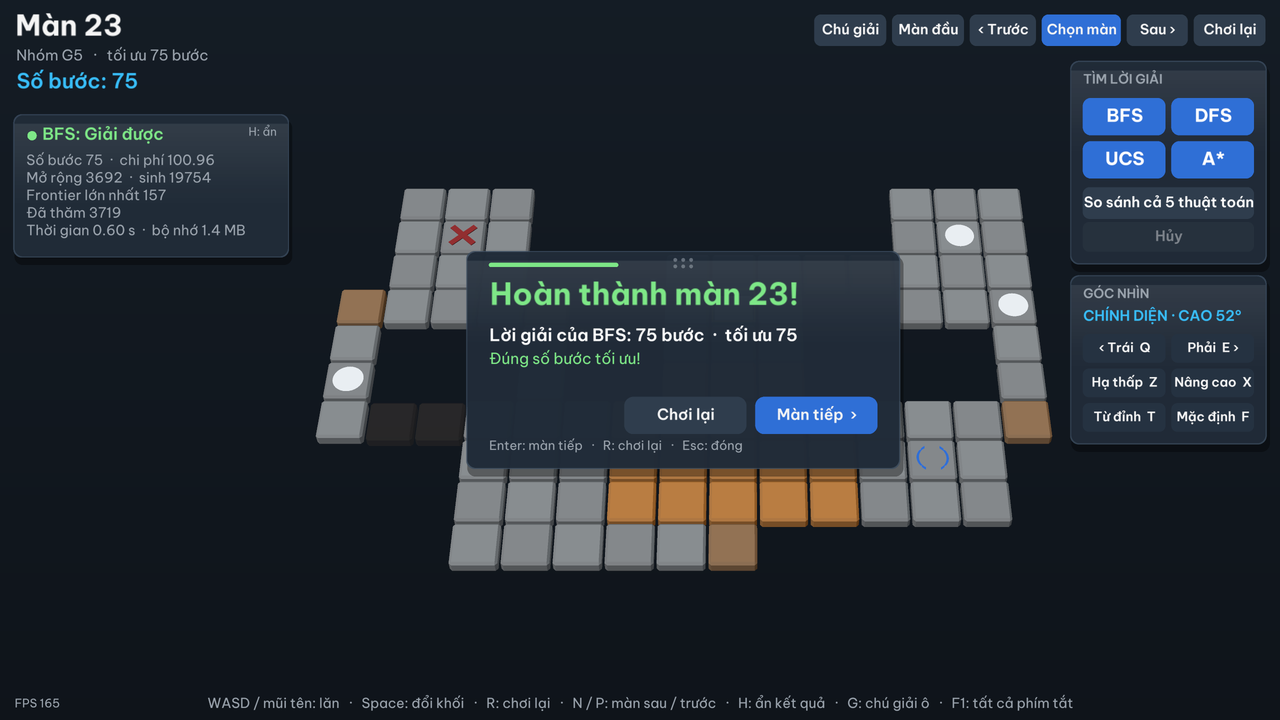
\includegraphics[width=0.86\linewidth,height=\textheight,keepaspectratio,alt={Hình 4.6}]{hinh/h4-6-giai-bfs-thang.png}
\caption{Hình 4.6. Màn 23 sau khi bấm Giải bằng BFS: khối đã tự lăn tới đích sau 75 bước, đúng số bước tối ưu; khung kết quả hiện các chỉ số của lần tìm, bàn thu nhỏ vào phần màn hình còn trống nên không bị che.}
\end{figure}

\textbf{So sánh} chạy lần lượt năm thuật toán trên màn đang mở: BFS, DFS, UCS, A* với \(h_P\) và A* với \(h_M\), mỗi thuật toán một tiến trình. Chạy lần lượt chứ không song song để thời gian và bộ nhớ của các thuật toán không ảnh hưởng nhau. Bảng được điền dần khi từng thuật toán xong (Hình 4.7, 4.8); dòng đang chạy ghi số giây đã chạy; thuật toán nào lỗi thì ô ghi ``Lỗi'' và nội dung lỗi ghi dưới bảng. Cột ``Giây'' và ``MB'' ghi số không kèm đơn vị cho bảng gọn.

\begin{figure}
\centering
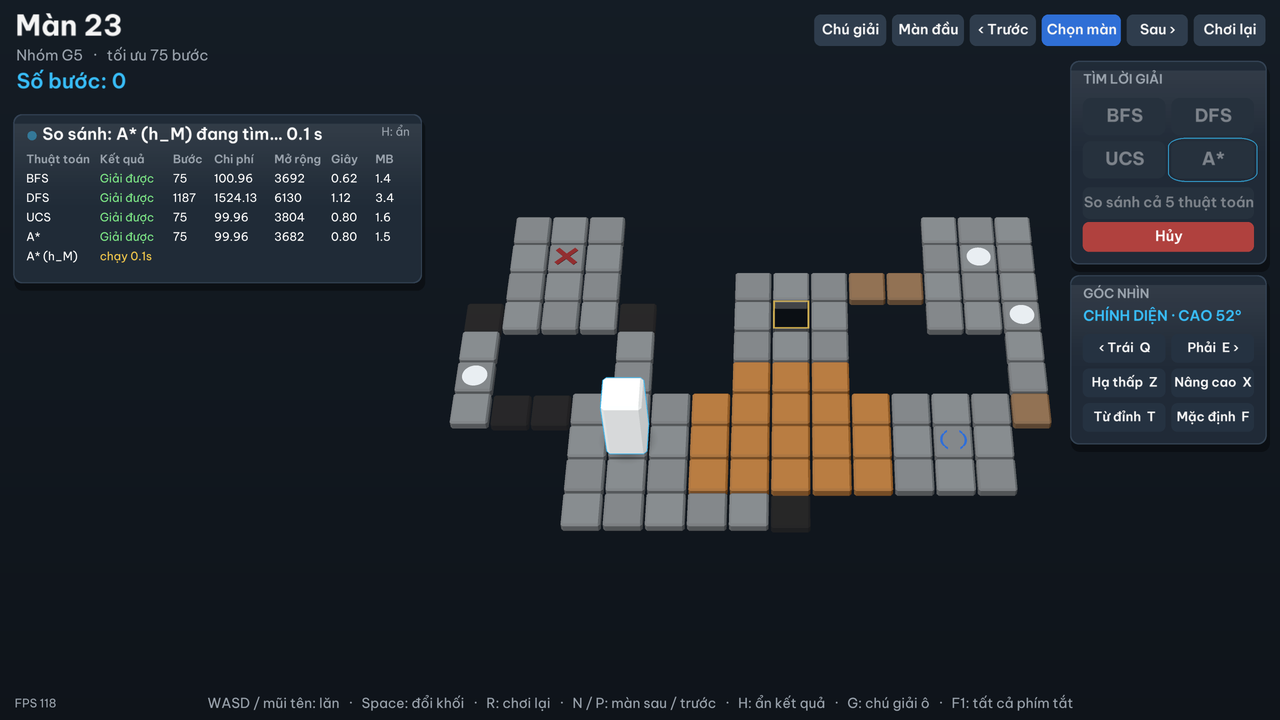
\includegraphics[width=0.86\linewidth,height=\textheight,keepaspectratio,alt={Hình 4.7}]{hinh/h4-7-so-sanh-dang-chay.png}
\caption{Hình 4.7. So sánh đang chạy trên màn 23: bốn thuật toán đã xong, A}
\end{figure}

\begin{figure}
\centering
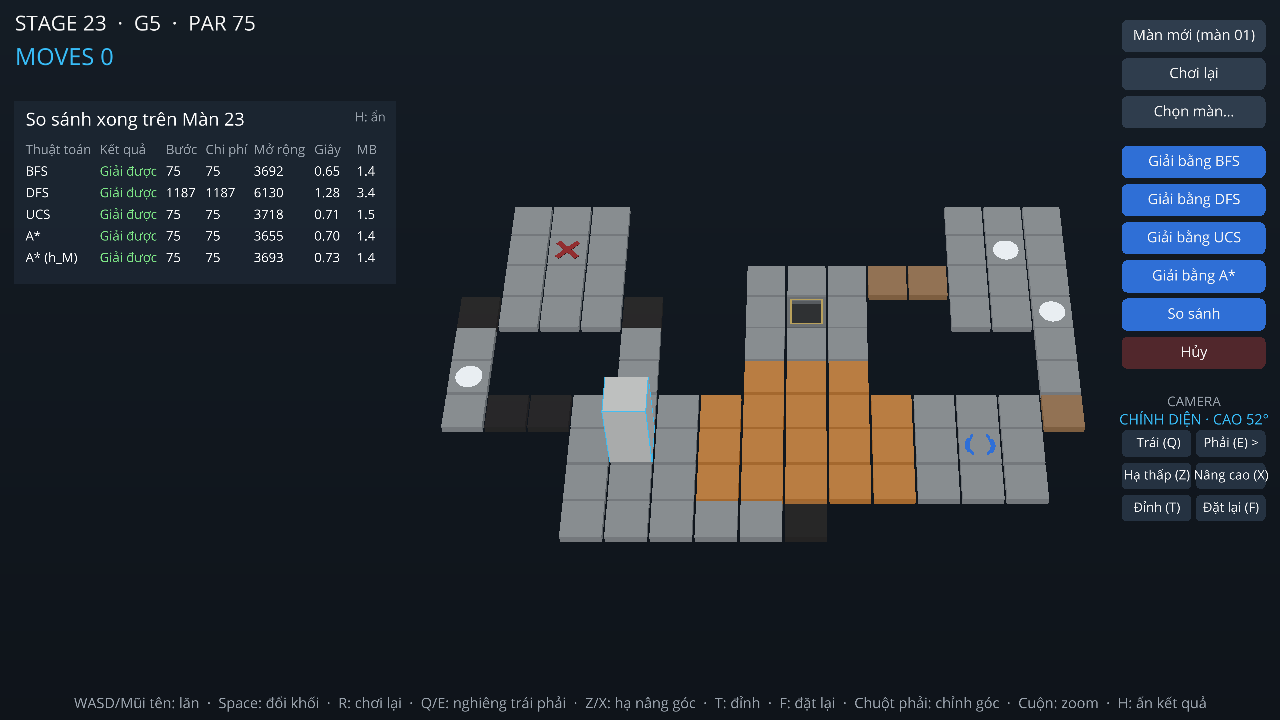
\includegraphics[width=0.86\linewidth,height=\textheight,keepaspectratio,alt={Hình 4.8}]{hinh/h4-8-so-sanh-xong.png}
\caption{Hình 4.8. Kết quả So sánh trên màn 23: BFS, UCS và A}
\end{figure}

Nút Giải và So sánh dựng bài toán với hàm chi phí ở mục 3.3, nên cột Chi phí của cả năm thuật toán tính theo cùng một hàm (mục 3.3.2): BFS cho số bước ít nhất, UCS và A* cho tổng chi phí nhỏ nhất. Ở màn 23, BFS đi 75 bước tốn 101,58, còn UCS và A* đi 75 bước khác tốn 100,58.

Thời gian và bộ nhớ trên giao diện chỉ để tham khảo, vì tiến trình con luôn bật \texttt{tracemalloc} để đo bộ nhớ, và việc này làm chậm thuật toán. Số liệu ở chương 5 lấy từ script thực nghiệm.

\begin{figure}
\centering
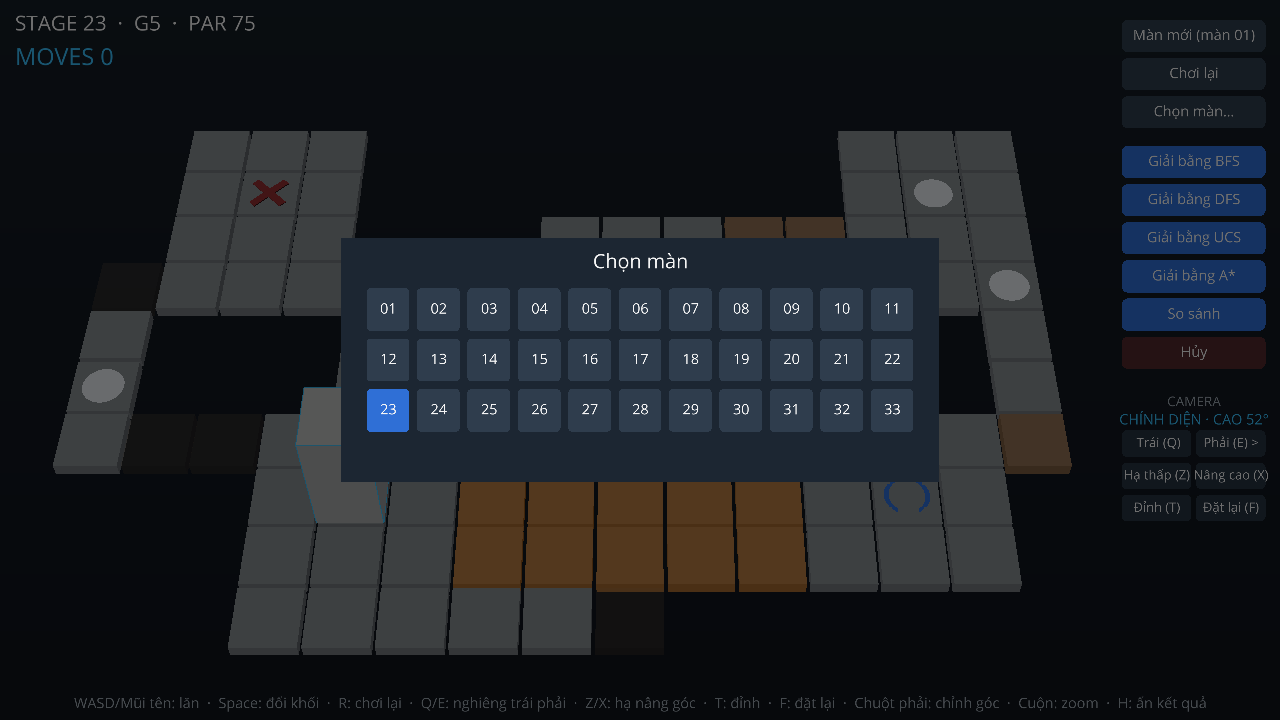
\includegraphics[width=0.86\linewidth,height=\textheight,keepaspectratio,alt={Hình 4.9}]{hinh/h4-9-chon-man.png}
\caption{Hình 4.9. Lưới chọn màn: màn đang mở tô màu xanh; bấm một mã màn để chuyển thẳng tới màn đó, thuật toán đang chạy (nếu có) bị hủy. Bấm ra ngoài lưới, Esc hoặc Ctrl+K để đóng. Màn đã thắng trong lần chạy này có chấm xanh ở góc nút.}
\end{figure}

\subsection{4.7. Camera và bố cục màn hình}

Camera xoay quanh tâm bàn và \textbf{luôn nhìn từ trên xuống, từ phía người chơi}. Nếu cho xoay tự do 360°, người chơi dễ lẫn hướng: khi camera quay quá 45°, phím ↑ không còn đẩy khối ``ra xa màn hình'' nữa. Vì vậy góc nhìn chỉ đổi trong vùng giới hạn (Hình 4.10):

\begin{itemize}
\tightlist
\item
  \textbf{Nghiêng trái, phải} (Q / E): năm nấc 40° trái, 20° trái, chính diện, 20° phải, 40° phải. Góc lệch luôn dưới 45° nên bốn phím mũi tên giữ nguyên nghĩa trên màn hình, giao diện không phải đổi lại hướng phím.
\item
  \textbf{Hạ thấp, nâng cao} (Z / X): góc giữa mặt bàn và hướng nhìn có bốn nấc 52°, 45°, 38°, 30°. Góc thấp thấy rõ khối đứng và độ cao của khối, góc cao thấy rõ toàn bàn; người chơi chọn nấc thấy dễ nhìn.
\item
  \textbf{Nhìn từ đỉnh} (T): nhìn thẳng xuống, bàn thẳng hàng với màn hình; bấm T lần nữa thì trở về góc trước đó. Góc đỉnh đặt 88,5° chứ không đúng 90° để phép tính hướng nhìn không bị suy biến.
\item
  \textbf{Kéo chuột phải} chỉnh góc liên tục nhưng vẫn trong vùng trên; \textbf{con lăn} thu phóng; \textbf{F} về góc mặc định (chính diện, 52°). Góc đã chọn được giữ khi đổi màn.
\end{itemize}

Camera chuyển góc mượt bằng nội suy mỗi khung hình. Khi nghiêng ngang, camera lùi xa thêm một chút vì bàn chiếm chỗ theo đường chéo; hướng ``lên'' của camera luôn ghim theo trục y nên hình không bị xoay nghiêng dần sau nhiều lần đổi góc. Tên góc đang dùng (ví dụ ``CHÍNH DIỆN · CAO 52°'') hiện trên nhóm nút camera.

\begin{figure}
\centering
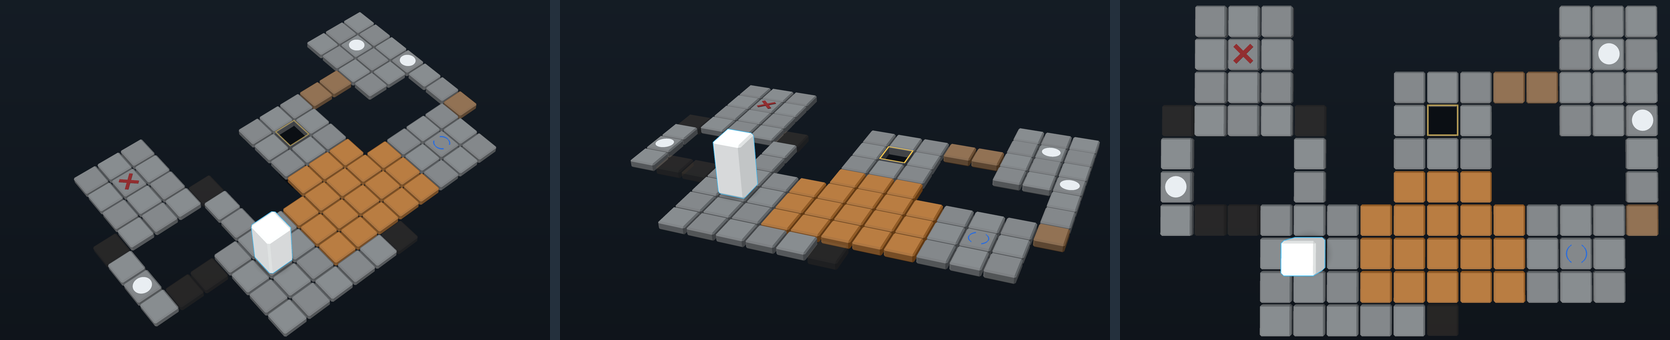
\includegraphics[width=0.86\linewidth,height=\textheight,keepaspectratio,alt={Hình 4.10}]{hinh/h4-10-goc-camera.png}
\caption{Hình 4.10. Màn 23 ở ba góc nhìn: nghiêng trái 40° (cao 52°), nghiêng phải 20° hạ thấp còn 30°, và nhìn từ đỉnh. Ở cả ba góc, phím ↑ vẫn đẩy khối về phía trên màn hình.}
\end{figure}

\textbf{Bố cục khi khung kết quả hiện.} Khung kết quả nằm ở cột bên trái, gọn theo nội dung: rộng vừa các chỉ số khi giải bằng một thuật toán, rộng vừa bảng khi So sánh (vị trí cột tính theo bề rộng chữ thật). Bàn chỉ bị dời hoặc thu khi thật sự bị khung che: giao diện chiếu các góc ô qua camera để biết bàn chiếm đoạn nào trên màn hình. Nếu bàn đã nằm ngoài khung thì giữ nguyên; nếu chạm khung thì ưu tiên dời ngang (bằng độ lệch ống kính, góc nhìn không đổi), chỉ khi dời không đủ mới lùi camera, và chỉ lùi vừa đủ để bàn nằm gọn giữa khung và cột nút (Hình 4.6, 4.8). Đổi góc camera trong lúc khung đang hiện thì bàn được đo và căn lại. Phím H ẩn khung; kết quả lần giải mới luôn hiện lại khung.

Khung kết quả, hộp kết thúc và các thẻ nút có nền hơi trong (vẫn thấy lờ mờ bàn phía sau), viền mảnh, một dải sáng rất nhẹ ở mép trên mờ dần xuống và bóng mềm phía dưới, để tách khỏi nền mà không che hẳn bàn.

\subsection{4.8. Kiểm thử giao diện}

Ngoài unit test của engine và thuật toán (không cần Ursina), giao diện được thử bằng các script mở cửa sổ thật và tự bấm phím, bấm nút thay người chơi. Các dòng có ghi 29/10 được chạy lại trên giao diện hiện tại; các dòng còn lại chạy ngày 23/10 và phần code liên quan chưa đổi từ đó.

{\def\LTcaptype{none} % do not increment counter
\begin{longtable}[]{@{}
  >{\raggedright\arraybackslash}p{(\linewidth - 2\tabcolsep) * \real{0.5660}}
  >{\raggedright\arraybackslash}p{(\linewidth - 2\tabcolsep) * \real{0.4340}}@{}}
\toprule\noalign{}
\begin{minipage}[b]{\linewidth}\raggedright
\textbf{Kiểm tra}
\end{minipage} & \begin{minipage}[b]{\linewidth}\raggedright
\textbf{Kết quả}
\end{minipage} \\
\midrule\noalign{}
\endhead
\bottomrule\noalign{}
\endlastfoot
Chơi tay theo lời giải BFS ở màn 2, 4, 8 (cầu, ô dễ vỡ, tách và ghép) & Thắng đúng 17, 28, 10 bước \\
Đứng lên ô dễ vỡ ở màn 4, rồi bấm R & Rơi, đúng thông báo; ô được dựng lại \\
Bấm R giữa lúc khối đang lăn & Không bị lượt cũ ghi đè \\
Giải bằng BFS rồi tự lăn, trên cả 33 màn (29/10) & 33/33 màn thắng đúng số bước tối ưu \\
Giải bằng DFS rồi tự lăn ở màn 1, 8, 16, 23, 29 & Thắng ở cả 5 màn (màn 23: 1187 bước) \\
So sánh trên cả 33 màn & 33/33 màn đủ năm dòng kết quả \\
So sánh trên màn 23 (29/10) & Đủ năm dòng; BFS, UCS, A* (\(h_P\)), A* (\(h_M\)) 75 bước, DFS 1187 bước \\
Bấm Hủy khi đang giải và khi đang So sánh; đổi màn khi đang giải & Dừng đúng; các nút trở lại trạng thái ban đầu \\
Đổi qua mọi nấc Q/E, Z/X, T rồi F (29/10) & Camera dừng đúng nấc, hình không bị xoay nghiêng; F về chính diện 52° \\
Khung kết quả hiện, rồi bấm H (29/10) & Bàn thu vào phần còn trống, không bị che; ẩn khung thì bàn về cỡ đầy đủ \\
Cài trong môi trường ảo mới theo README & Cài đúng phiên bản, test qua, cửa sổ mở được \\
Giải bằng BFS rồi tự lăn trên cả 33 màn, với hoạt ảnh lật khối mới (30/10) & 33/33 màn thắng đúng số bước tối ưu \\
Bấm phím ngẫu nhiên mỗi khung hình (lăn, R, N, P, Space, camera, Ctrl+K) xen với Giải, So sánh, Hủy; 17 lần × 35 giây (30/10) & Không lỗi, không treo (trước khi sửa hoạt ảnh hẹn giờ: 4/12 lần dừng vì lỗi \texttt{!is\_\allowbreak{}empty()}) \\
Kéo hộp kết thúc bằng chuột (giả lập), kéo ra ngoài màn hình, bấm vào nút trong hộp (30/10) & Hộp đi theo chuột, dừng ở mép màn hình; bấm nút không kéo hộp; lần thắng sau hộp hiện ở chỗ đã kéo \\
Khung kết quả hiện ở màn 23 (một thuật toán, rồi So sánh) (30/10) & Bàn giữ nguyên cỡ khi không bị che; khi So sánh chỉ thu vừa đủ \\
Thắng ở màn 1; bấm F1, Esc; rơi ở màn 1 (30/10) & Khối thu vừa miệng lỗ và nhìn thấy trong lòng lỗ; hộp thắng ghi đúng số bước; hộp rơi ghi đúng lý do \\
Lăn ra mép ở màn 1 (một đầu hụt, rồi hụt cả hai đầu), tách và ghép ở màn 8, đứng lên ô dễ vỡ, rồi bấm R (30/10) & Khối đổ nghiêng qua mép, không xuyên sàn; chỉ khối con hụt rơi; ô dễ vỡ được dựng lại \\
Rà soát giao diện: Hủy khi khối tự lăn, bấm R khi cầu đang đổi, Giải/So sánh ngay sau khi rơi, chữ trong khung kết quả, Enter khi mở F1, thu phóng khi khung hiện (30/10) & 6 lỗi tái hiện được trước khi sửa, không còn sau khi sửa \\
Bảng chú giải: G, nút ``Chú giải'', Esc, F1 khi bảng đang mở; Enter và phím lăn khi bảng đang mở (31/10) & Mở, đóng đúng; F1 thay bảng chú giải; Enter và phím lăn bị bỏ qua \\
\end{longtable}
}

\subsection{4.9. Hạn chế}

\begin{itemize}
\tightlist
\item
  Chấm đánh dấu màn đã thắng chỉ giữ trong một lần chạy chương trình, chưa lưu ra file.
\item
  Chưa chỉnh được tốc độ khối tự lăn và chưa tạm dừng được giữa chừng (chỉ dừng hẳn bằng Hủy hoặc R).
\item
  Menu chọn màn chỉ có 33 màn gốc; bộ màn tự sinh S1--S3 (chương 5) chưa mở được từ giao diện.
\end{itemize}
